%Title: Fus. evap results for U and Th isotopes
%Author: A. Raggio
%Year: 2020

\documentclass[10pt]{beamer}

%
%Setting file
%

\usepackage[T1]{fontenc}
\usepackage[utf8]{inputenc}

\usepackage[english]{babel}

\usepackage{graphicx}
\graphicspath{{images/}}
\usepackage{float}
\usepackage{tikz}
\usepackage{caption}
\usepackage{subcaption}

\usetheme{default}
\usefonttheme{structurebold}


% ---------------------------------
% color definitions
\usepackage{color}
% \definecolor{LISA_BLUE}{rgb}{0.25,0.33,0.66}
\definecolor{LISA_BLUE}{cmyk}{0.99,0.88,0.29,0.18}

\setbeamercolor{normal text}{fg=LISA_BLUE}
\setbeamercolor{frametitle}{fg=LISA_BLUE}

\newcommand\insertlocation{}  % Empty by default.
\newcommand\location[1]{\renewcommand\insertlocation{#1}}

\newcommand\insertperiod{}  % Empty by default.
\newcommand\period[1]{\renewcommand\insertperiod{#1}}



\setbeamertemplate{itemize items}[circle]
\setbeamercolor{title}{fg=white}



%-----------------------------------------Title page settings-----------------------------------------%
\title{\normalsize I262 Setup Detection Efficiency}

\institute{}

\author{}

%\author{%
%\begin{columns}
%\column{.48\textwidth}%
%Candidate:
%Andrea Raggio.
%\hfill%
%\column{.48\textwidth}%
%Supervisor:
%Daniele Mengoni
%\end{columns}
%}

\date{}
\titlegraphic{% 
\vspace{0.05\textheight}
	\centering
	
\includegraphics[height=3cm]{jyu-keskitetty-kaksikielinen.eps}\\
\vspace{-0.03\textheight}
}
%-----------------------------------------Title page settings-----------------------------------------%


\setbeamertemplate{footline}
{
 \begin{beamercolorbox}{section in head/foot}
 \vskip2pt\hspace{0.095cm} Andrea Raggio \hfill Jyv\"{a}skyl\"{a} - November 2020 \hspace{0.15cm}\phantom{x}\vskip2pt
 \end{beamercolorbox}%
}


\begin{document}
\frame{\titlepage}

\begin{frame}{BEGE Efficiency}
	
	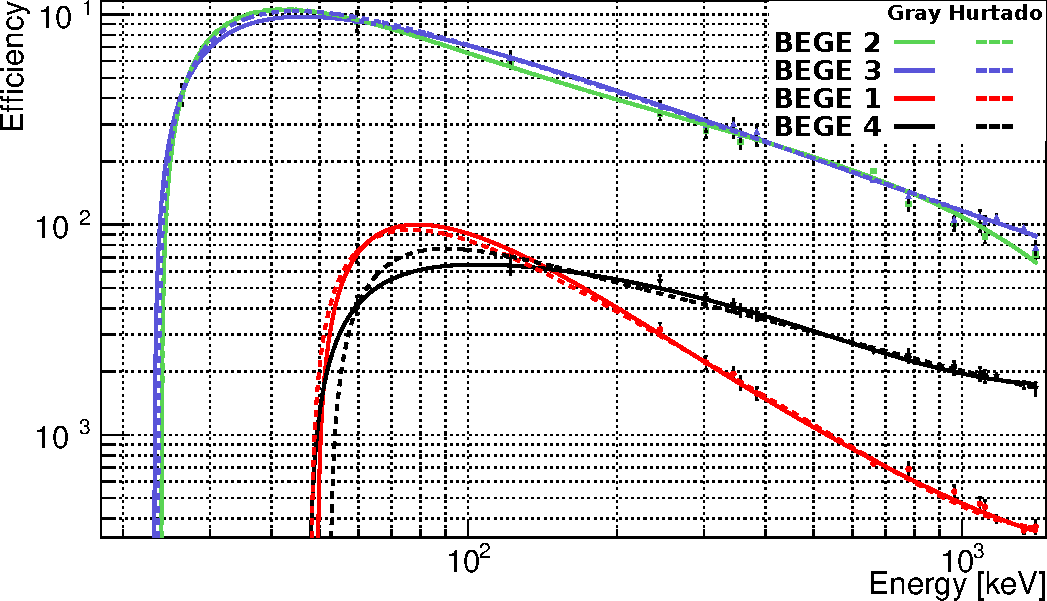
\includegraphics[width=\textwidth]{BEGE_final.pdf}
	\small
	\textcolor{red}{Gray 80–1850 keV \hfill  Hurtado 36–1500 keV}

\end{frame}


\begin{frame}{Si Efficiency}
	\vspace{-0.1\textheight}
	\begin{columns}
		\begin{column}{0.5\textwidth}
			\begin{overlayarea}{\textwidth}{0.5\textheight}
				\centering
				\textbf{QuadSi1}
				\vspace{-0.05\textheight}
				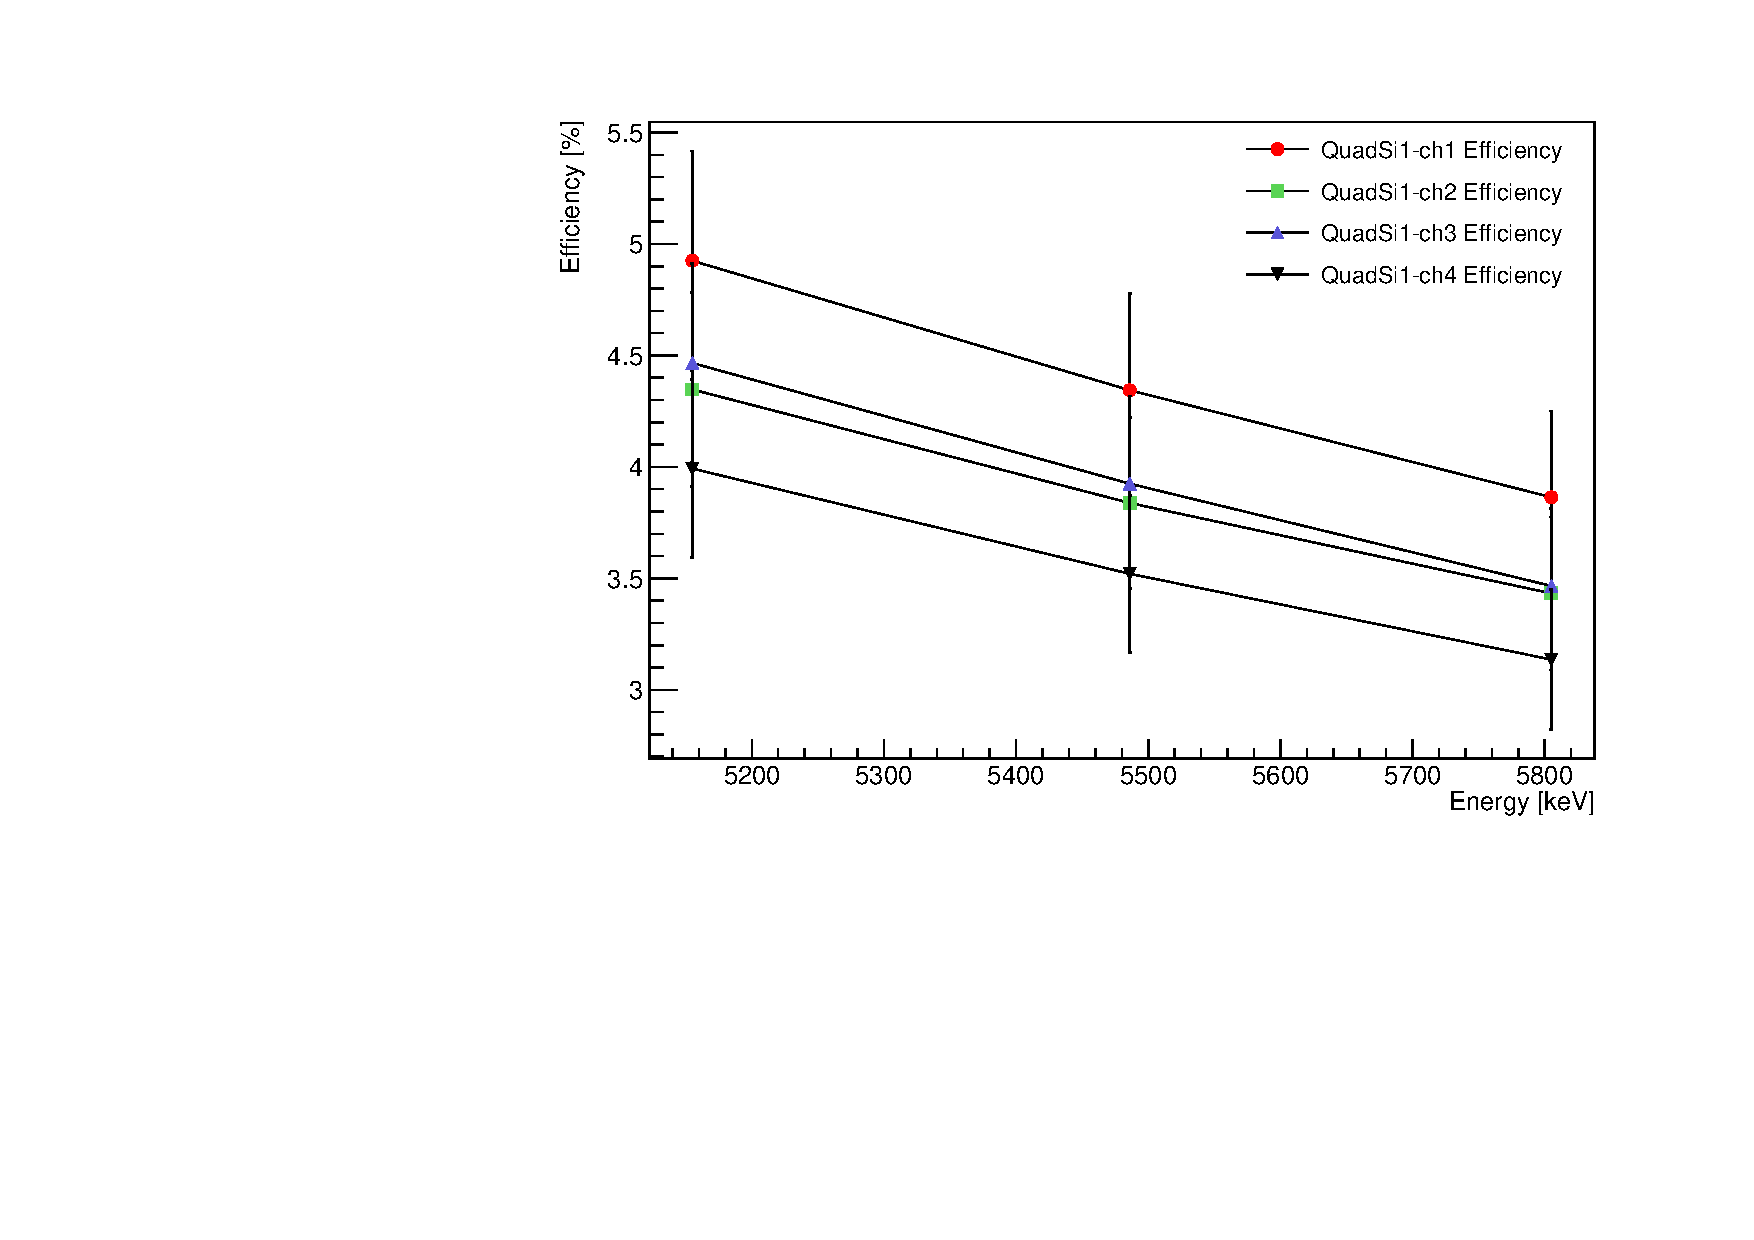
\includegraphics[width=0.95\textwidth]{QuadSi1.pdf}
			\end{overlayarea}
		\end{column}
		\begin{column}{0.5\textwidth}
			\begin{overlayarea}{\textwidth}{0.5\textheight}
				\centering
				\textbf{QuadSi2}
				\vspace{-0.05\textheight}
				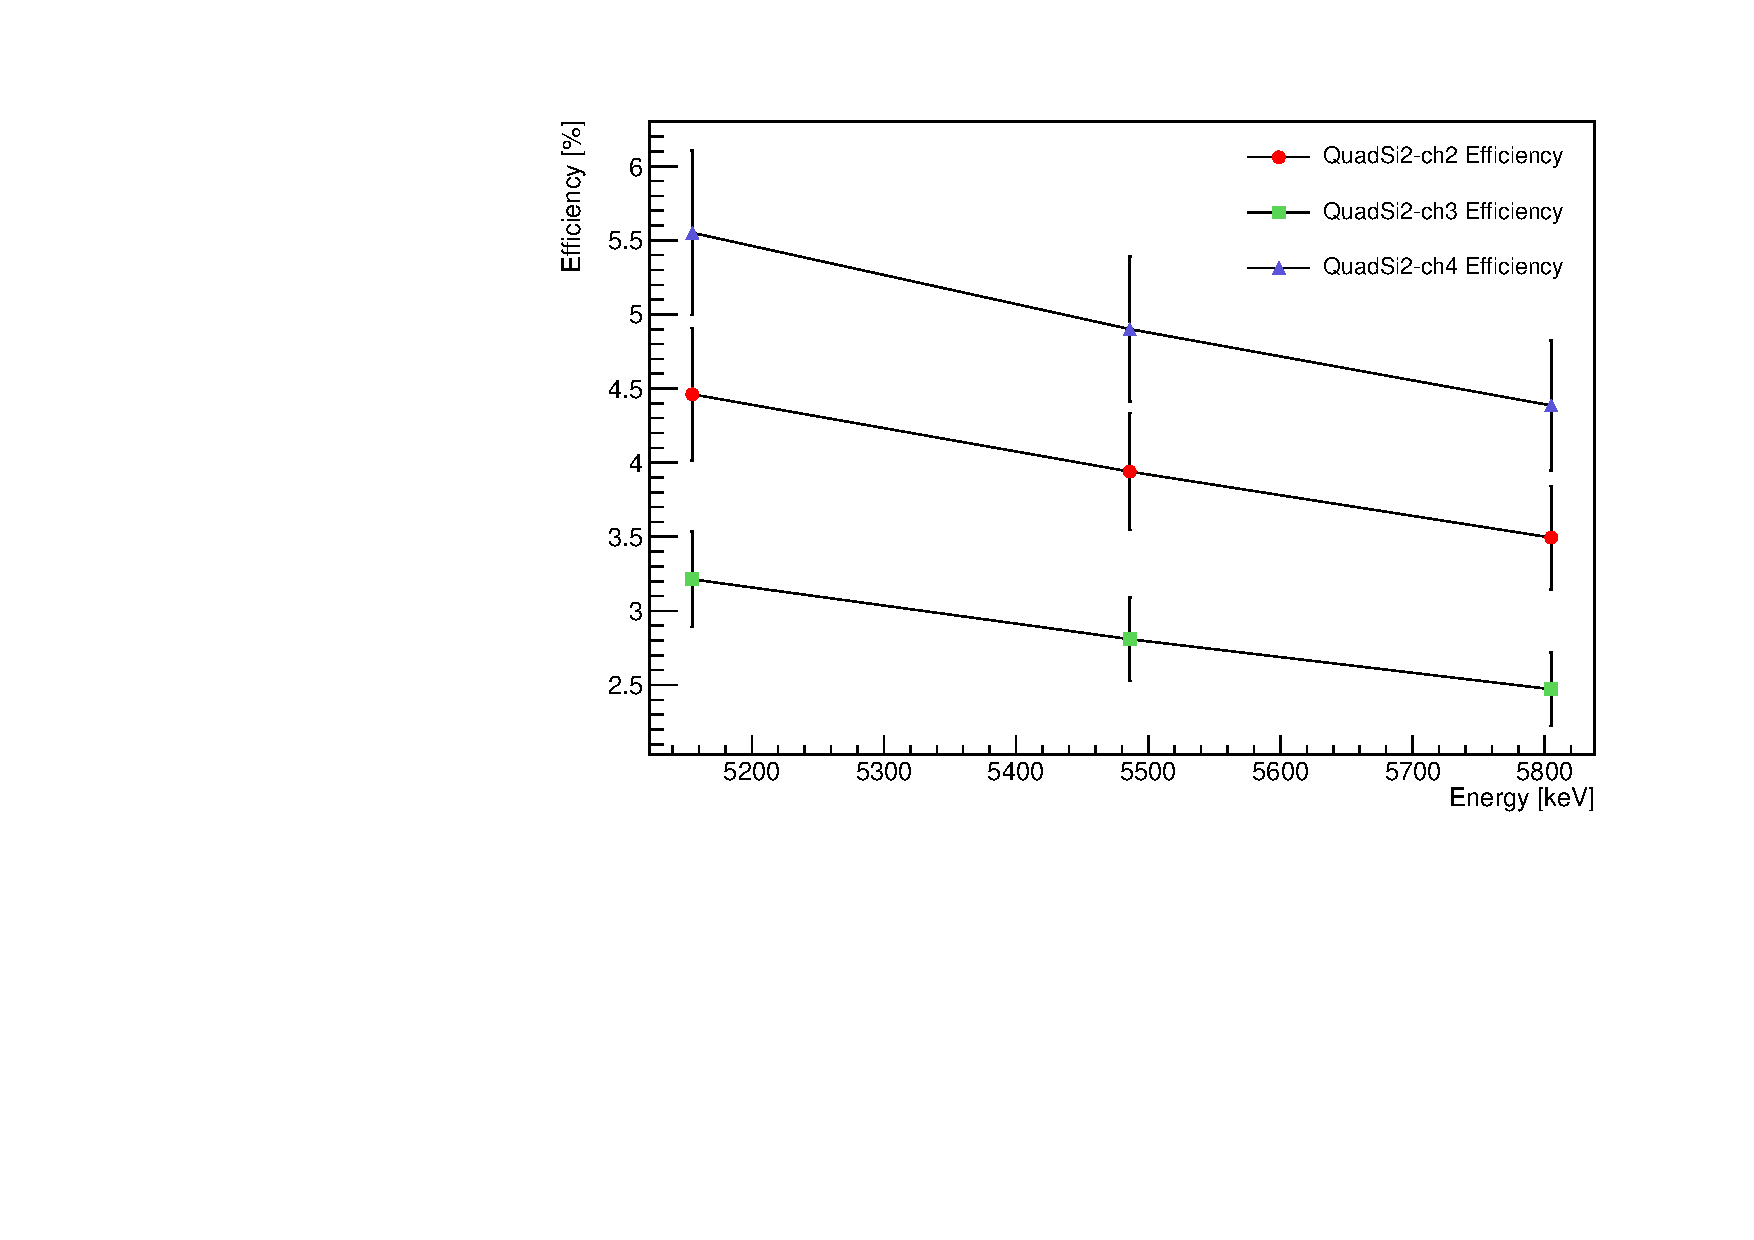
\includegraphics[width=0.95\textwidth]{QuadSi2.pdf}
			\end{overlayarea}
		\end{column}
	\end{columns}	
	\centering
	\textbf{Si(Li) + CircSi}\\
	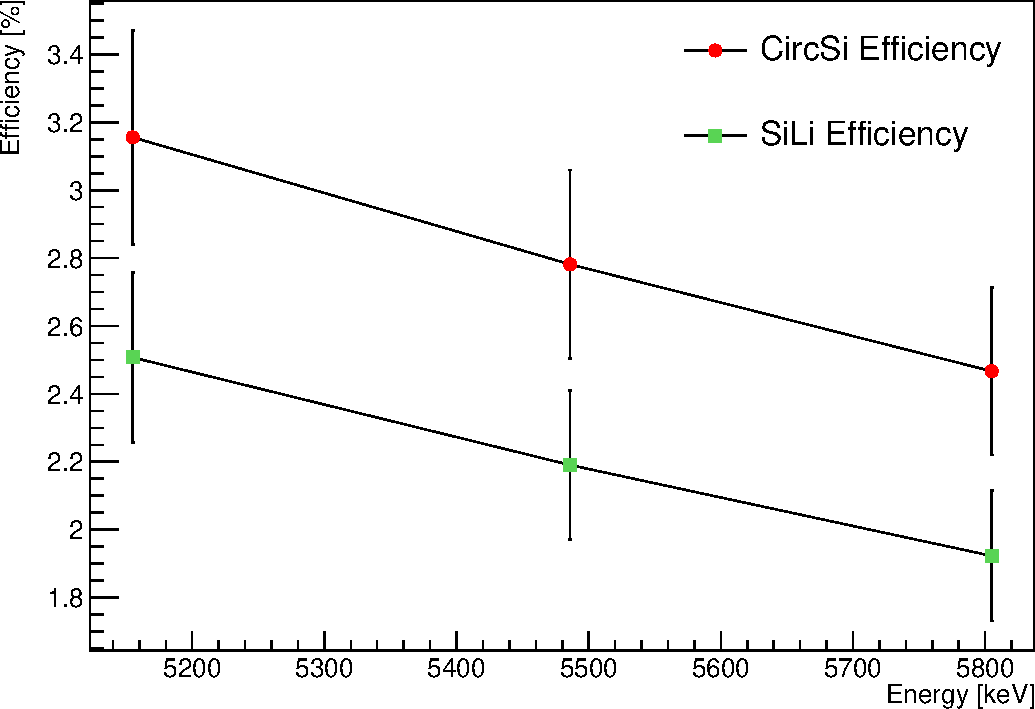
\includegraphics[width=0.4\textwidth]{SiLi_CircSi.pdf}

\end{frame}

\end{document}